\documentclass[12pt, a4paper]{article}
\usepackage[utf8]{inputenc} 
\usepackage[margin=1.2in]{geometry}
%\usepackage{multicol}
%\usepackage{multirow}
%\usepackage{url}
\usepackage{graphicx}
%\usepackage{xcolor}
%\usepackage{amsfonts}
\usepackage[tbtags]{amsmath}
%\usepackage{amsfonts,amssymb,amsmath,graphicx}
\usepackage{tikz}
\usetikzlibrary{arrows}
%\usepackage{caption}
\usepackage{subcaption}
\usepackage{float}
\usepackage{forest}
\definecolor{lightpurple}{HTML}{D8BFD8}
\definecolor{skyblue}{RGB}{135,206,235}
\tikzset{root/.style={circle, draw=blue!60, fill=blue!5, very thick, minimum size=7mm},
	min/.style={circle, draw=blue!60, fill=blue!20, very thick, minimum size=7mm},
	marked/.style={circle, draw=red!60, fill=red!5, very thick, minimum size=7mm}
}
\usepackage{indentfirst}


\usetikzlibrary{shapes.geometric}
\tikzstyle{non_marked_node} = [draw, circle, text width=.3cm, thick, fill=blue!30, text centered]
\tikzstyle{marked_node} = [draw, circle, text width=.3cm, thick, fill=gray!30, text centered]
\tikzstyle{target_node} = [draw, circle, text width=.3cm, thick, fill=red!30, text centered]

\title{
	\line(1,0){300}
	\endgraf\bigskip
	\Huge
	\begin{center}
		\emph{\Large{\textbf{Fibonacci Heap: A Data Structure Used for Improved Network Optimization Algorithms}}}
		
	\end{center}
	\line(1,0){300}
	\bigskip
	\bigskip
}

\author{
	\textbf{Jarin Tasneem}\\Student ID: 2005019\\
	\textbf{Swastika Pandit}\\Student ID: 2005027\\
	\textbf{Fairuz Mubashwera}\\Student ID: 2005030\\\\
	Department of Computer Science and Engineering\\
	Bangladesh University of Engineering and Technology\\
}

\date{
	\endgraf\bigskip
	{\today}
}

\begin{document}

	\maketitle
	\pagenumbering{roman}
	\pagebreak
	
	\tableofcontents
	\setcounter{tocdepth}{2}
	\newpage
	
	\listoffigures
	\newpage
	
	%  \listoftables
	%  \newpage
	
	
	\pagenumbering{arabic}
	\section{Introduction}
	Fibonacci heap is a data structure for implementing priority queues. It is an optimized extension of binomial heap. While binomial heap supports all heap operations in $O(log n)$ worst case time complexity for a n-item heap, Fibonacci heap supports arbitrary deletion in $O(log n)$ amortized time, and all other heap operations in $O(log n)$ time. It is particularly useful where number of insert and decrease-key operations is significantly larger than delete and extract-min operations.
	
	\section{History of Using Heap structures in Computer Science}
	
	
	In the 1960s, heaps were introduced as a data structure in computer science. Initially, the term "heap" referred to a memory region used for dynamic memory allocation. This era marked the inception of structured heap data structures, laying the foundation for their evolution in subsequent decades.
	
	The 1970s witnessed the rise of binary heaps, including both binary min-heaps and max-heaps, as fundamental data structures. Their efficient representation using arrays and straightforward operations made them integral for implementing priority queues, significantly impacting algorithm design and efficiency during this period.
	
	In the 1980s, Bernard O. Tree introduced binomial heaps, a notable advancement in heap structures. Binomial heaps addressed certain limitations of binary heaps, providing more efficient merge operations. These heaps found applications in various algorithms, notably contributing to the optimization of Dijkstra's shortest path algorithm.
	
	\begin{table}[h]
		\centering
		\begin{tabular}{c c}
			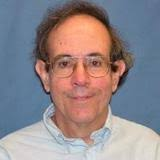
\includegraphics[scale=0.7]{History/Michael.jpg} & 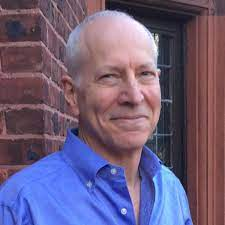
\includegraphics[scale=0.5]{History/Tarjan.jpg} \\
		\end{tabular}
	\end{table}
	\captionof{figure}{Michael L. Fredman and Robert E. Tarjan}
	
	
	A pivotal moment occurred in 1986 when Michael L. Fredman and Robert E. Tarjan introduced Fibonacci Heaps through their paper \textit{"Fibonacci Heaps and Their Uses."} Designed to enhance the efficiency of decrease key operations, Fibonacci Heaps proved particularly suitable for algorithms such as Dijkstra's and Prim's. This marked a significant milestone in the ongoing evolution of heap data structures, showcasing the continual quest for optimized solutions in computer science.
	
	
	\section{Motivation}
	
	
	\subsection*{A Comparison with Other Data Structures}
	\begin{table}[h]
		\centering
		\begin{tabular}{|c|c|c|c|}
			\hline
			\textbf{Operation}& \textbf{Binary heap} & \textbf{Binomial heap} & \textbf{Fibonacci heap} \\
			\hline
			Insert & O(log(n)) & O(log(n)) & O(1)\\
			\hline
			Decrease key & O(log(n)) & O(log(n)) & O(1)\\
			\hline
			Extract min & O(log(n)) & O(log(n)) & O(log(n))\\
			\hline
			Delete & O(log(n)) & O(log(n)) & O(log(n))\\
			\hline
			Find min& O(1) & O(log(n)) & O(1)\\
			\hline
			Union & O(n) & O(log(n)) & O(1)\\
			\hline
		\end{tabular}
		\caption{Time complexity comparison of Fibonacci heap with other heap structures}
		\label{tab:my_label1}
		
	\end{table} 
	\vspace{5mm}
	
	In binomial heap, most of the operations can be done in $O(log n)$ time. But when we try to extract-min or delete, decrease key operation is needed to often. Since in binomial heap, each decrease-key operation would need a heapify operation of time-complexity $O(log n)$, the overall performance becomes slow. To solve this problem, Fibonacci heap was introduced, where the prime motivation was to gain $O(1)$ amortized time-complexity in decrease-key operation.\newline
	
	Fibonacci heap structure is much more relaxed and less strict than binomial heap data structure. Due to "Lazy Consolidation" we can merge and decrease a key without having to heapify in each of these operations. Owing to this feature and relaxation in its structure, Fibonacci heap has been able to bring significant performance improvement in optimization of graph and network algorithms.\cite{fredman1987fibonacci}
	
	\section{Structure}
	\begin{itemize}
		\item A Fibonacci heap is a collection of item-disjoint \textit{heap-ordered trees} \\
		A heap-ordered tree is a rooted tree where for any node \textit{x}, the key of the children of \textit{x} is no less than key of \textit{x}, provided \textit{x} has children. Thus the root contains the minimum key node.
		\item The number of children of a node is called its \textit{rank r(x)}.
		\item Each node is either \textit{marked} or \textit{unmarked}. \cite{fredman1987fibonacci}  
	\end{itemize}
	\begin{figure}[!h]
		\centering
		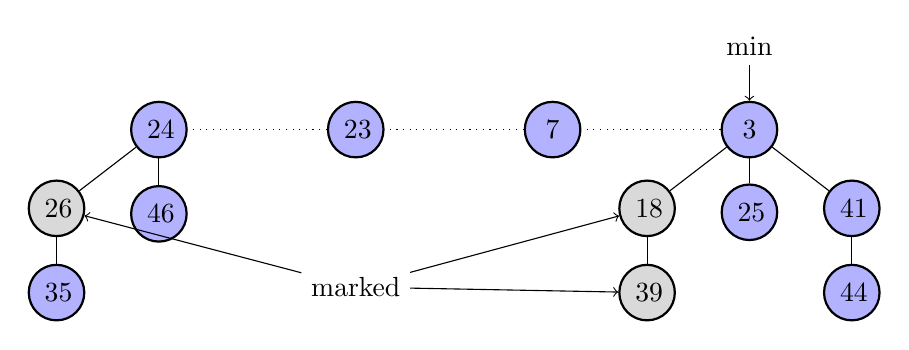
\begin{tikzpicture}
			\centering
			\node[non_marked_node](3){3};
			\node[marked_node, left of=3, yshift=-1cm, xshift=-.3cm](18) {18};
			\node[non_marked_node, below of=3, yshift=-.05cm](25) {25};
			\node[non_marked_node, right of=3, yshift=-1cm, xshift=.3cm](41) {41};
			\node[marked_node, below of=18, yshift=-.07cm](39) {39};
			\node[non_marked_node, below of=41, yshift=-0.07cm](44) {44};
			\node[non_marked_node, left of=3, xshift=-1.5cm](7){7};
			\node[non_marked_node, left of=7, xshift=-1.5cm](23){23};
			\node[non_marked_node, left of=23, xshift=-1.5cm](24){24};
			\node[marked_node, left of=24, xshift=-0.3cm, yshift=-1cm](26) {26};
			\node[non_marked_node, below of=24, yshift=-.07cm](46) {46};
			\node[non_marked_node, below of=26, yshift=-.07cm] (35) {35};
			
			% draw lines
			\draw (3) -- (18) node [near start, above]{};
			\draw (3) -- (25) node [near start, above]{}; 
			\draw (3) -- (41) node [near start, above]{};
			\draw (18) -- (39) node [near start, above]{};
			\draw (41) -- (44) node [near start, above]{};
			\draw (24) -- (26) node [near start, above]{};
			\draw (24) -- (46) node [near start, above]{};
			\draw (26) -- (35) node [near start, above]{};
			\draw[dotted] (3.west) -- (7.east) node [near start, above]{};
			\draw[dotted] (7.west) -- (23.east) node [near start, above]{};
			\draw[dotted] (23.west) -- (24.east) node [near start, above]{};
			
			\node[above of=3, yshift=.06cm] (min) {min};
			\draw[black, ->] (min.south) -- (3.north);
			\node[below of=23, yshift=-1cm] (marked) {marked};
			\draw[black, ->] (marked) -- (18) node [near start, above]{};
			\draw[black, ->] (marked) -- (39) node [near start, above]{};
			\draw[black, ->] (marked) -- (26) node [near start, above]{};
		\end{tikzpicture}
		\caption{A Fibonacci heap}
		%\label{fig:enter-label}
	\end{figure}
	
	\pagebreak
	\section{Memory Representation of the Nodes of Fibonacci Heap}
	\begin{itemize}
		\item Each node contains a pointer to its parent (or \textit{null} if it has no parent) and a pointer to one of its children.
		\item The children of each are stored in a doubly-linked list.
		\item Each node contains its rank, and a bit to indicate whether it is marked.
		\item The roots of all the trees in a heap are stored in a doubly-linked list.
		\item Heap is accessed by a pointer to a root containing an item of minimum key, which is called the \textit{minimum node} of heap. A minimum node of null indicates an empty heap.
	\end{itemize}
	
	\begin{figure}[!h]
		\centering
		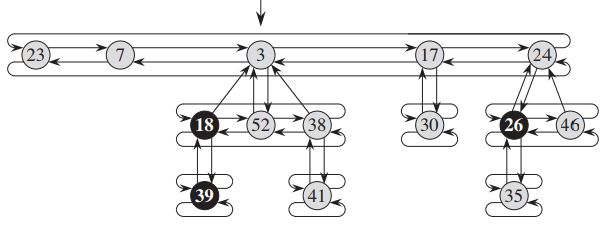
\includegraphics[]{pointers.png}
		\caption{complete representation showing pointers p (up arrows), child (down arrows), and left and right
			(sideways arrows)\cite{cormen2022introduction}.}
	\end{figure}
	
	
	\section{Fibonacci Heap Operations}
	Fibonacci heap offers a diverse array of operations, comparable to other common structures like binary heaps and binomial heaps. Some of the most common operations associated with Fibonacci heaps are:
	
	\begin{itemize}
		\item Make-Heap
		\item Insert
		\item Union
		\item Find-min
		\item Extract-Min
		\item Decrease-key
		\item Delete
	\end{itemize}
	
	We'll see implementations of each operation one by one.

	
	\subsection{Make-Heap}
	This operation creates an empty heap. A heap is represented by a single tree rooted at the minimum element in the heap. Initially, this tree is empty.
	
	\subsection{Insert}
	This operation adds a new element to the heap. The new element is added as a single tree rooted at the new element and linked to the existing trees in the heap. The minimum element of the tree is compared to the newly inserted element. If the new element is smaller than the element pointed by \textit{min pointer}, then the \textit{min pointer} is updated to point to the new element, otherwise it remains unchanged.
	
	\begin{itemize}
		\item Make a new tree with the new key.
		\begin{figure}[!h]
			\centering  
			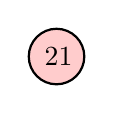
\begin{tikzpicture}
				\node[non_marked_node, fill=red!20](21){21};
			\end{tikzpicture}
		\end{figure}
		\begin{figure}% Start minipage
			\centering			
			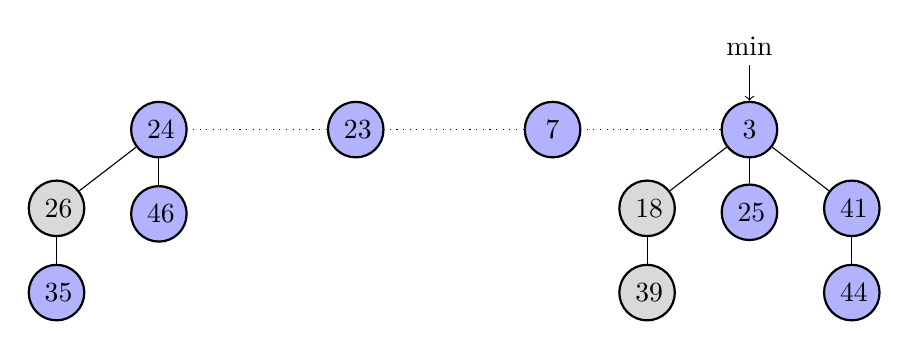
\begin{tikzpicture}
				\node[non_marked_node](3){3};
				\node[marked_node, left of=3, yshift=-1cm, xshift=-.3cm](18) {18};
				\node[non_marked_node, below of=3, yshift=-.05cm](25) {25};
				\node[non_marked_node, right of=3, yshift=-1cm, xshift=.3cm](41) {41};
				\node[marked_node, below of=18, yshift=-.07cm](39) {39};
				\node[non_marked_node, below of=41, yshift=-0.07cm](44) {44};
				\node[non_marked_node, left of=3, xshift=-1.5cm](7){7};
				\node[non_marked_node, left of=7, xshift=-1.5cm](23){23};
				\node[non_marked_node, left of=23, xshift=-1.5cm](24){24};
				\node[marked_node, left of=24, xshift=-0.3cm, yshift=-1cm](26) {26};
				\node[non_marked_node, below of=24, yshift=-.07cm](46) {46};
				\node[non_marked_node, below of=26, yshift=-.07cm] (35) {35};
				
				% draw lines
				\draw (3) -- (18) node [near start, above]{};
				\draw (3) -- (25) node [near start, above]{}; 
				\draw (3) -- (41) node [near start, above]{};
				\draw (18) -- (39) node [near start, above]{};
				\draw (41) -- (44) node [near start, above]{};
				\draw (24) -- (26) node [near start, above]{};
				\draw (24) -- (46) node [near start, above]{};
				\draw (26) -- (35) node [near start, above]{};
				\draw[dotted] (3.west) -- (7.east) node [near start, above]{};
				\draw[dotted] (7.west) -- (23.east) node [near start, above]{};
				\draw[dotted] (23.west) -- (24.east) node [near start, above]{}; 
				\node[above of=3, yshift=.06cm] (min) {min};
				\draw[black, ->] (min.south) -- (3.north);       
			\end{tikzpicture}
			\captionof{figure}{In this example, 21 is the new key to be inserted in the Fibonacci heap. A new tree is created with a single node 21.}
			\label{fig:enter-label}
		\end{figure} % End minipage
		
		\item Add the new tree to the heap (usually next to the min pointer).
		\item Update the min pointer if required.\\
		\begin{minipage}{\linewidth} % Start minipage
			\centering
			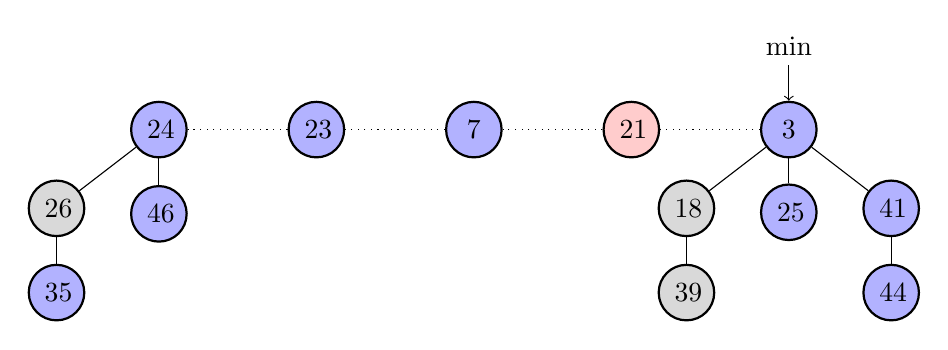
\begin{tikzpicture}
				\node[non_marked_node](3){3};
				\node[marked_node, left of=3, yshift=-1cm, xshift=-.3cm](18) {18};
				\node[non_marked_node, below of=3, yshift=-.05cm](25) {25};
				\node[non_marked_node, right of=3, yshift=-1cm, xshift=.3cm](41) {41};
				\node[marked_node, below of=18, yshift=-.07cm](39) {39};
				\node[non_marked_node, below of=41, yshift=-0.07cm](44) {44};
				\node[non_marked_node, left of=3, xshift=-1cm, fill=red!20](21){21};
				
				\node[non_marked_node, left of=21, xshift=-1cm](7){7};
				
				\node[non_marked_node, left of=7, xshift=-1cm](23){23};
				\node[non_marked_node, left of=23, xshift=-1cm](24){24};
				\node[marked_node, left of=24, xshift=-0.3cm, yshift=-1cm](26) {26};
				\node[non_marked_node, below of=24, yshift=-.07cm](46) {46};
				\node[non_marked_node, below of=26, yshift=-.07cm] (35) {35};
				
				% draw lines
				\draw (3) -- (18) node [near start, above]{};
				\draw (3) -- (25) node [near start, above]{}; 
				\draw (3) -- (41) node [near start, above]{};
				\draw (18) -- (39) node [near start, above]{};
				\draw (41) -- (44) node [near start, above]{};
				\draw (24) -- (26) node [near start, above]{};
				\draw (24) -- (46) node [near start, above]{};
				\draw (26) -- (35) node [near start, above]{};
				\draw[dotted] (3.west) -- (21.east) node [near start, above]{};
				\draw[dotted] (21.west) -- (7.east) node [near start, above]{};
				\draw[dotted] (7.west) -- (23.east) node [near start, above]{};
				\draw[dotted] (23.west) -- (24.east) node [near start, above]{}; 
				\node[above of=3, yshift=.06cm] (min) {min};
				\draw[black, ->] (min.south) -- (3.north);       
			\end{tikzpicture}
			\captionof{figure}{The newly created tree is added to the Fibonacci heap. Since 21 is greater than min node 3, no need to update the min-pointer}
			\label{fig:enter-label}
		\end{minipage} % End minipage
	\end{itemize}
	
	\subsection{Union}
	
	Union operation takes two Fibonacci heaps H1 and H2 and merges them to one heap H\\
	\begin{minipage}{\linewidth}
		\centering
		\begin{forest}
			for tree={
				if level=1{no edge}{}, 
				if level=0{}{draw},
				if n children=0{fit=band}{},
				circle, inner sep=0pt, minimum size=1.7em,
				tier/.pgfmath=level(), s sep=.5cm
			}
			[
			[23, root, name=23
			[11, non_marked_node]
			]
			[24, root, name=24 
				[50, non_marked_node		[60, non_marked_node]]
				[46, non_marked_node]
			]
			[17, root, name=17]
			[7, root, name=7]
			[3, root, name=3
				[18, non_marked_node [39, non_marked_node]]
				[25, non_marked_node]
				[30, non_marked_node	 [44, non_marked_node]]]
			[21, root, name=21]
			]
			\draw[black, thick, ->, dotted] (23) to [out=east, in=west] (24);
			\draw[black, thick, ->, dotted] (24) to [out=east, in=west] (17);
			\draw[black, thick, ->, dotted] (7) to [out=east, in=west] (3);	
			\draw[black, thick, ->, dotted] (3) to [out=east, in=west] (21);
			\draw[black, thick, ->, dotted] (17) to [out=north, in=north] (23);
			\draw[black, thick, ->, dotted] (21) to [out=north, in=north] (7);
			\node[above of=3, yshift=.06cm] (min) {min};
			\draw[black, ->] (min.south) -- (3.north);
			\node[above of=17, yshift=.06cm] (min2) {min};
			\draw[black, ->] (min2.south) -- (17.north);
			\node[draw, circle, text width=.3cm, thick, draw=white, below of=24, yshift=-3cm](H1) {H1};
			\node[draw, circle, text width=.3cm, thick, draw=white, below of=3, yshift=-3cm](H2) {H2};			
		\end{forest}
		\caption{Two heaps H1 and H2.}
	\end{minipage} % End minipage
	\begin{itemize}
		
		\item  Merge the two rootlists (usually rootlists are stored in a doubly-linked list)
		\begin{minipage}{\linewidth} % Start minipage
			\centering
			\begin{forest}
				for tree={
					if level=1{no edge}{}, 
					if level=0{}{draw},
					if n children=0{fit=band}{},
					circle, inner sep=0pt, minimum size=1.7em,
					tier/.pgfmath=level(), s sep=.5cm
				}
				[
				[23, root, name=23
				[11, non_marked_node]
				]
				[24, root, name=24 
				[50, non_marked_node		[60, non_marked_node]]
				[46, non_marked_node]
				]
				[17, root, name=17]
				[7, root, name=7]
				[3, root, name=3
				[18, non_marked_node [39, non_marked_node]]
				[25, non_marked_node]
				[30, non_marked_node	 [44, non_marked_node]]]
				[21, root, name=21]
				]
				\draw[black, thick, ->, dotted] (23) to [out=east, in=west] (24);
				\draw[black, thick, ->, dotted] (24) to [out=east, in=west] (17);
				\draw[black, thick, ->, dotted] (7) to [out=east, in=west] (3);	
				\draw[black, thick, ->, dotted] (3) to [out=east, in=west] (21);
				\draw[black, thick, ->, dotted] (17) to [out=north, in=north] (23);
				\draw[black, thick, ->, dotted] (21) to [out=north, in=north] (7);
				\node[above of=3, yshift=.06cm] (min) {min};
				\draw[black, ->] (min.south) -- (3.north);
				\node[draw, circle, text width=.3cm, thick, draw=white, below of=24, yshift=-3cm](H1) {H1};
				\node[draw, circle, text width=.3cm, thick, draw=white, below of=3, yshift=-3cm](H2) {H2};			
			\end{forest}
			\captionof{figure}{Root lists are merged together to form a single heap H}
			\label{fig:enter-label}
		\end{minipage} % End minipage
		\item  Make the min pointer with smaller value the min pointer of the merged heap.
	\end{itemize}
	
	
	\subsection{Find-min}
	The find-min operation in a Fibonacci heap is a simple operation that returns the minimum key value in the heap without removing it. In the basic structure of Fibonacci heap, we have a min pointer that always points to the updated minimum value of the entire heap. 
	
	\begin{minipage}{\linewidth}
		\centering
		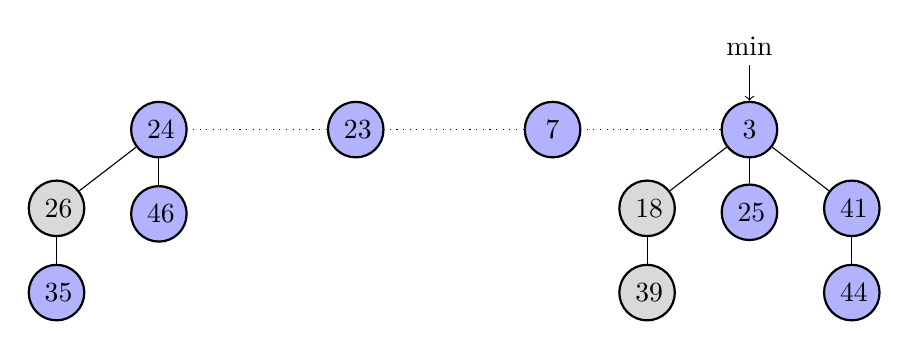
\begin{tikzpicture}
			\node[non_marked_node](3){3};
			\node[marked_node, left of=3, yshift=-1cm, xshift=-.3cm](18) {18};
			\node[non_marked_node, below of=3, yshift=-.05cm](25) {25};
			\node[non_marked_node, right of=3, yshift=-1cm, xshift=.3cm](41) {41};
			\node[marked_node, below of=18, yshift=-.07cm](39) {39};
			\node[non_marked_node, below of=41, yshift=-0.07cm](44) {44};
			\node[non_marked_node, left of=3, xshift=-1.5cm](7){7};
			\node[non_marked_node, left of=7, xshift=-1.5cm](23){23};
			\node[non_marked_node, left of=23, xshift=-1.5cm](24){24};
			\node[marked_node, left of=24, xshift=-0.3cm, yshift=-1cm](26) {26};
			\node[non_marked_node, below of=24, yshift=-.07cm](46) {46};
			\node[non_marked_node, below of=26, yshift=-.07cm] (35) {35};
			
			% draw lines
			\draw (3) -- (18) node [near start, above]{};
			\draw (3) -- (25) node [near start, above]{}; 
			\draw (3) -- (41) node [near start, above]{};
			\draw (18) -- (39) node [near start, above]{};
			\draw (41) -- (44) node [near start, above]{};
			\draw (24) -- (26) node [near start, above]{};
			\draw (24) -- (46) node [near start, above]{};
			\draw (26) -- (35) node [near start, above]{};
			\draw[dotted] (3.west) -- (7.east) node [near start, above]{};
			\draw[dotted] (7.west) -- (23.east) node [near start, above]{};
			\draw[dotted] (23.west) -- (24.east) node [near start, above]{}; 
			\node[above of=3, yshift=.06cm] (min) {min};
			\draw[black, ->] (min.south) -- (3.north);       
		\end{tikzpicture}
		\caption{A Fibonacci heap with a min-pointer pointed to the minimum value}
		\label{fig:enter-label}
	\end{minipage}
	\vspace{5mm}
	In find-min operation, we just return the minimum value pointed by the min-pointer.
	
	\subsection{Decrease-key}
	
	An amortized time complexity O(1) in case of completing decrease-key operation was the prime motivation behind the introduction of Fibonacci heap data structure. The major two obstacles of achieving this goal was 
	
	\begin{enumerate}
		\item Decreasing a key might break the heap property
		\item Preserving heap property after any operation needs an extra heapify operation that take $O(log n)$ running time
	\end{enumerate}
	
	To solve these two issues, decrease-key operation of Fibonacci heap is described differently than that of other heaps. The steps generally followed are:
	
	\begin{enumerate}
		
		\item If the decreased node violates the heap order, cut the sub-tree rooted at the note and add it to the root list.
		\item Since the newly added sub-tree has a minimum value as its node, no need to heapify. Problem Solved in O(1) amortized time!
	\end{enumerate}
	\vspace{5mm}
	Let's see a simulation of decrease-key. 
	
	\begin{minipage}{\linewidth}
		\centering
		\begin{forest}
			for tree={
				if level=1{no edge}{}, 
				if level=0{}{draw},
				if n children=0{fit=band}{},
				circle, inner sep=0pt, minimum size=1.7em,
				tier/.pgfmath=level(), s sep=.5cm
			}
			[
			[7, non_marked_node, name=7
				[23, non_marked_node
					[26, marked_node
						[34, non_marked_node]	[90, non_marked_node]
					]
					[45, target_node
						[72, non_marked_node]]]
				[17, non_marked_node
					[30, non_marked_node]]
				[23, non_marked_node]
			]
			[18, non_marked_node, marked_node, name=18
				[21, non_marked_node
					[51, non_marked_node]
				]
				[39, non_marked_node]
			]
			[37, non_marked_node, name=37
				[59, non_marked_node]
			]
			]
			\draw [black, thick, dotted] (7) to [out=east, in=west] (18);
			\draw [black, thick, dotted] (18) to [out=east, in=west] (37);
			\node[above of=7, yshift=.06cm] (min) {min};
			\draw[black, ->] (min.south) -- (7.north);
		\end{forest}
		\caption{In this Fibonacci heap, the node 45 will be decreased with a smaller value 15}
		\label{fig:enter-label}
	\end{minipage}
	
	\begin{itemize}
		\item \textbf{Decrease a Key with Smaller Value:}
	\end{itemize}
	
	
	\begin{minipage}{\linewidth} % Start minipage
		\centering
		\begin{forest}
			for tree={
				if level=1{no edge}{}, 
				if level=0{}{draw},
				if n children=0{fit=band}{},
				circle, inner sep=0pt, minimum size=1.7em,
				tier/.pgfmath=level(), s sep=.5cm
			}
			[
			[7, non_marked_node, name=7
			[23, non_marked_node
			[26, marked_node
			[34, non_marked_node]	[90, non_marked_node]
			]
			[15, target_node
			[72, non_marked_node]]]
			[17, non_marked_node
			[30, non_marked_node]]
			[23, non_marked_node]
			]
			[18, non_marked_node, marked_node, name=18
			[21, non_marked_node
			[51, non_marked_node]
			]
			[39, non_marked_node]
			]
			[37, non_marked_node, name=37
			[59, non_marked_node]
			]
			]
			\draw [black, thick, dotted] (7) to [out=east, in=west] (18);
			\draw [black, thick, dotted] (18) to [out=east, in=west] (37);
			\node[above of=7, yshift=.06cm] (min) {min};
			\draw[black, ->] (min.south) -- (7.north);
		\end{forest}
		\caption{A violation of heap order.}
		\label{fig:enter-label}
	\end{minipage}
	
	\begin{itemize}
		\item \textbf{Cut the Rooted Subtree and Add it to Root-list:}
	\end{itemize}
	
	\begin{minipage}{\linewidth} % Start minipage
		\centering
		\begin{forest}
			for tree={
				if level=1{no edge}{}, 
				if level=0{}{draw},
				if n children=0{fit=band}{},
				circle, inner sep=0pt, minimum size=1.7em,
				tier/.pgfmath=level(), s sep=.5cm
			}
			[
			[15, target_node, name=15
			[72, non_marked_node]]
			[7, non_marked_node, name=7
			[23, marked_node
			[26, marked_node
			[34, non_marked_node]	[90, non_marked_node]
			]
			]
			[17, non_marked_node
			[30, non_marked_node]]
			[23, non_marked_node]
			]
			[18, non_marked_node, marked_node, name=18
			[21, non_marked_node
			[51, non_marked_node]
			]
			[39, non_marked_node]
			]
			[37, non_marked_node, name=37
			[59, non_marked_node]
			]
			]
			\draw [black, thick, dotted] (7) to [out=east, in=west] (18);
			\draw [black, thick, dotted] (18) to [out=east, in=west] (37);
			\draw [black, thick, dotted] (15) to [out=east, in=west] (7);
			\node[above of=7, yshift=.06cm] (min) {min};
			\draw[black, ->] (min.south) -- (7.north);
		\end{forest}
		\caption{The subtree rooted at 15 is cut and added as a new tree to the root-list.}
		\label{fig:enter-label}
	\end{minipage} 
	\vspace{5mm}
	
	In this process the parent, 23 of the root, 15 of the cut subtree was marked. 
	
	\subsubsection{Why parents need to be marked when a child is cut?}
	
	So that we can keep a maximum degree of a node bounded. If the degree of a node is not bounded, a node can have as many children as possible.\newline
	
	\begin{minipage}{\linewidth} % Start minipage
		\centering
		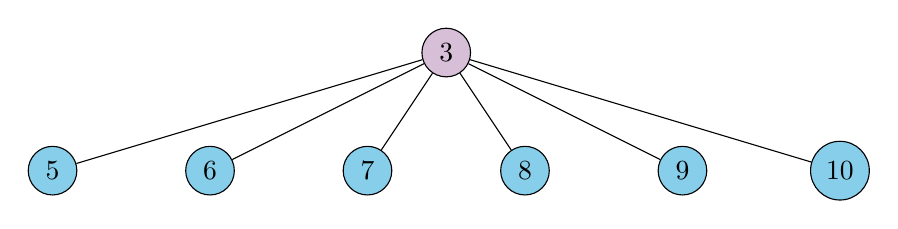
\begin{tikzpicture}[level distance=1.5cm,
			level 1/.style={sibling distance=2cm},
			level 2/.style={sibling distance=2cm}]
			\node[circle,draw,fill=lightpurple] (root) {3}
			child {node[circle,draw,fill=skyblue] {5}}
			child {node[circle,draw,fill=skyblue] {6}}
			child {node[circle,draw,fill=skyblue] {7}}
			child {node[circle,draw,fill=skyblue] {8}}
			child {node[circle,draw,fill=skyblue] {9}}
			child {node[circle,draw,fill=skyblue] {10}};
		\end{tikzpicture}
		\caption{A problematic structure if maximum degree of a not is not bounded}
		
	\end{minipage}\newline
	
	In this example, root 3 has 6 children. This kind of structure would significantly impact the performance increasing it to O(n) of many operations like decrease-key, extract-min, delete etc. Cascading cut prevents these kind of structures.
	\begin{itemize}
		\item Nodes are initially unmarked.
		\item When a child is cut from a node, the node becomes marked.
		\item If a child is cut from a marked node, cut the marked node itself and do it recursively.\newline
	\end{itemize}
	
	Let's see a simulation of cascading cut!
	
	\begin{minipage}{\linewidth}
		
		\centering
		\begin{forest}
			for tree={
				if level=1{no edge}{}, 
				if level=0{}{draw},
				if n children=0{fit=band}{},
				circle, inner sep=0pt, minimum size=1.7em,
				tier/.pgfmath=level(), s sep=.5cm
			}
			[
			[15, non_marked_node, name=15
			[72, non_marked_node]]
			[7, non_marked_node, name=7
			[23, marked_node
			[10, target_node
			[34, non_marked_node]	[90, non_marked_node]
			]
			]
			[17, non_marked_node
			[30, non_marked_node]]
			[23, non_marked_node]
			]
			[18, non_marked_node, marked_node, name=18
			[21, non_marked_node
			[51, non_marked_node]
			]
			[39, non_marked_node]
			]
			[37, non_marked_node, name=37
			[59, non_marked_node]
			]
			]
			\draw [black, thick, dotted] (7) to [out=east, in=west] (18);
			\draw [black, thick, dotted] (18) to [out=east, in=west] (37);
			\draw [black, thick, dotted] (15) to [out=east, in=west] (7);
			\node[above of=7, yshift=.06cm] (min) {min};
			\draw[black, ->] (min.south) -- (7.north);
		\end{forest}
		\caption{Cascading cut: Child cut from a marked node 23}
		\label{fig:enter-label}
		
	\end{minipage}
	
	\begin{itemize}
		\item An already marked node 23 is losing another child. So we need to cut this node 23 as well and make it a newly added tree. This is called recursively cascading cut.
	\end{itemize}
	
	\begin{minipage}{\linewidth}
		
		\centering
		\begin{forest}
			for tree={
				if level=1{no edge}{}, 
				if level=0{}{draw},
				if n children=0{fit=band}{},
				circle, inner sep=0pt, minimum size=1.7em,
				tier/.pgfmath=level(), s sep=.5cm
			}
			[
			[23, marked_node, name=23]
			[10, target_node, name=10
			[34, non_marked_node]	[90, non_marked_node]
			]
			[15, non_marked_node, name=15
			[72, non_marked_node]]
			[7, marked_node, name=7			
			[17, non_marked_node
			[30, non_marked_node]]
			[23, non_marked_node]
			]
			[18, non_marked_node, marked_node, name=18
			[21, non_marked_node
			[51, non_marked_node]
			]
			[39, non_marked_node]
			]
			[37, non_marked_node, name=37
			[59, non_marked_node]
			]
			]
			\draw [black, thick, dotted] (7) to [out=east, in=west] (18);
			\draw [black, thick, dotted] (18) to [out=east, in=west] (37);
			\draw [black, thick, dotted] (15) to [out=east, in=west] (7);
			\draw [black, thick, dotted] (23) to [out=east, in=west] (10);
			\draw [black, thick, dotted] (10) to [out=east, in=west] (15);
			\node[above of=7, yshift=.06cm] (min) {min};
			\draw[black, ->] (min.south) -- (7.north);
		\end{forest}
		\caption{Cascading cut: Marked node is cut as well.}
		\label{fig:enter-label}
		
	\end{minipage} 
	
	
	
	\subsection{Extract-min}
	"Extract-min" is one of the key operations of Fibonacci heap, which removes the minimum node from the heap.As this data structure maintains "lazy union",union operation happens after extract-min.The process is-\\
	
	\begin{enumerate}
		\item \textbf{Find the Minimum Node:} Traverse the root list of the Fibonacci Heap to find the node with the minimum key. This node represents the minimum element in the heap.\\
		
		\begin{minipage}{\linewidth} % Start minipage
			\centering
			\begin{forest}
				for tree={
					if level=1{no edge}{}, 
					if level=0{}{draw},
					if n children=0{fit=band}{},
					circle, inner sep=0pt, minimum size=1.7em,
					tier/.pgfmath=level(), s sep=.5cm
				}
					[
					[7, non_marked_node, name=7
						[30, non_marked_node]
					]
					[24, non_marked_node, name=24
						[26, marked_node
							[35, non_marked_node]]
						[46, non_marked_node]
					]
					[23, non_marked_node, name=23]
					[17, non_marked_node, name=17]
					[3, non_marked_node, name=3
						[18, non_marked_node
							[39, marked_node]]
						[52, non_marked_node]]
					]
					\draw [black, thick, dotted] (7) to [out=east, in=west] (24);
					\draw [black, thick, dotted] (24) to [out=east, in=west] (23);
					\draw [black, thick, dotted] (23) to [out=east, in=west] (17);
					\draw [black, thick, dotted] (17) to [out=east, in=west] (3);
					\node[above of=3, yshift=.06cm] (min) {min};
					\draw[black, ->] (min.south) -- (3.north);
			\end{forest}
			\captionof{figure}{A Fibonacci heap with minimum node 3}
			\label{fig:enter-label}
		\end{minipage} % End minipage
		
		\item \textbf{Remove Minimum Node from Root List:} Remove the minimum node from the root list of the heap. This involves updating the pointers of its neighboring nodes to bypass the node being removed.\\
		
		
		\item \textbf{Merge Children with Root List:} Combine the children of the minimum node with the root list. This step involves updating the pointers of the minimum node's children to remove the parent link and then merging the resulting list with the root list.\\
		
		\begin{minipage}{\linewidth} % Start minipage
			\centering
			\begin{forest}
				for tree={
					if level=1{no edge}{}, 
					if level=0{}{draw},
					if n children=0{fit=band}{},
					circle, inner sep=0pt, minimum size=1.7em,
					tier/.pgfmath=level(), s sep=.5cm
				}
				[
				[7, non_marked_node, name=7
				[30, non_marked_node]
				]
				[24, non_marked_node, name=24
				[26, marked_node
				[35, non_marked_node]]
				[46, non_marked_node]
				]
				[23, non_marked_node, name=23]
				[17, non_marked_node, name=17]
				[18, non_marked_node, name=18
				[39, marked_node]]
				[52, non_marked_node, name=52]
				]
				\draw [black, thick, dotted] (7) to [out=east, in=west] (24);
				\draw [black, thick, dotted] (24) to [out=east, in=west] (23);
				\draw [black, thick, dotted] (23) to [out=east, in=west] (17);
				\draw [black, thick, dotted] (17) to [out=east, in=west] (18);
				\draw [black, thick, dotted] (18) to [out=east, in=west] (52);
			\end{forest}
			\captionof{figure}{Removing minimum node and merging its children}
			\label{fig:enter-label}
		\end{minipage} % End minipage
		
		\item \textbf{Consolidate Trees:} After merging the children with the root list, there might be multiple trees with the same degree (number of children) in the root list. To ensure the Fibonacci Heap maintains its structural properties, consolidate these trees by combining trees of the same degree. During this process, a table (array) is used to keep track of trees with different degrees.\\
		
		\item \textbf{Update Minimum Pointer:} Traverse the consolidated root list to find the new minimum node and update the minimum pointer accordingly.
		
		\item \textbf{Update Marked Status:} If necessary, update the marked status of nodes in the consolidated heap. A node in a Fibonacci Heap is marked when it loses a child during a decrease key operation. This information is used to maintain the amortized time complexity of the decrease key operation.
		
		\begin{minipage}{\linewidth} % Start minipage
			\centering
			\begin{forest}
				for tree={
					if level=1{no edge}{}, 
					if level=0{}{draw},
					if n children=0{fit=band}{},
					circle, inner sep=0pt, minimum size=1.7em,
					tier/.pgfmath=level(), s sep=.5cm
				}
				[
				[7, non_marked_node, name=7
				[30, non_marked_node]
				]
				[24, non_marked_node, name=24
				[26, marked_node
				[35, non_marked_node]]
				[46, non_marked_node]
				]
				[23, non_marked_node, name=23]
				[17, non_marked_node, name=17]
				[18, non_marked_node, name=18
				[39, marked_node]]
				[52, non_marked_node, name=52]
				]
				\draw [black, thick, dotted] (7) to [out=east, in=west] (24);
				\draw [black, thick, dotted] (24) to [out=east, in=west] (23);
				\draw [black, thick, dotted] (23) to [out=east, in=west] (17);
				\draw [black, thick, dotted] (17) to [out=east, in=west] (18);
				\draw [black, thick, dotted] (18) to [out=east, in=west] (52);				
				\node [draw, rectangle, fit=(23) (17)](merge) {};
				\node[above of=merge, yshift=.06cm] (merge_text) {merge};
				\draw[black, ->] (merge_text.south) -- (merge.north);
				\node[below of=23, yshift=-2cm] (a) {(a)};
			\end{forest}
			\newline
			\begin{forest}				
				for tree={
					if level=1{no edge}{}, 
					if level=0{}{draw},
					if n children=0{fit=band}{},
					circle, inner sep=0pt, minimum size=1.7em,
					tier/.pgfmath=level(), s sep=.5cm
				}
				[
				[7, non_marked_node, name=7
				[30, non_marked_node]
				]
				[24, non_marked_node, name=24
				[26, marked_node
				[35, non_marked_node]]
				[46, non_marked_node, name=46]
				]
				[17, non_marked_node, name=17
					[23, non_marked_node, name=23]]
				[18, non_marked_node, name=18
				[39, marked_node]]
				[52, non_marked_node, name=52]
				]
				\draw [black, thick, dotted] (7) to [out=east, in=west] (24);
				\draw [black, thick, dotted] (24) to [out=east, in=west] (17);
				\draw [black, thick, dotted] (17) to [out=east, in=west] (18);
				\draw [black, thick, dotted] (18) to [out=east, in=west] (52);				
				\node [draw, rectangle, fit=(17) (23) (18) (17)](merge) {};
				\node[above of=merge, yshift=.7cm] (merge_text) {merge};
				\draw[black, ->] (merge_text.south) -- (merge.north);
				\node[below of=23, yshift=-1cm] (b) {(b)};
			\end{forest} 
			\newline
			\begin{forest}
				for tree={
					if level=1{no edge}{}, 
					if level=0{}{draw},
					if n children=0{fit=band}{},
					circle, inner sep=0pt, minimum size=1.7em,
					tier/.pgfmath=level(), s sep=.5cm
				}
				[
				[7, non_marked_node, name=7
				[30, non_marked_node]
				]
				[24, non_marked_node, name=24
				[26, marked_node, name=26
				[35, non_marked_node, name=35]]
				[46, non_marked_node]
				]
				[17, non_marked_node, name=17
				[23, non_marked_node, name=23]
				[18, non_marked_node, name=18
				[39, marked_node]]]				
				[52, non_marked_node, name=52]
				]
				\draw [black, thick, dotted] (7) to [out=east, in=west] (24);
				\draw [black, thick, dotted] (24) to [out=east, in=west] (17);
				\draw [black, thick, dotted] (17) to [out=east, in=west] (52);
				\node [draw, rectangle, fit=(24) (35) (18) (26)](merge) {};
				\node[above of=merge, yshift=1.4cm] (merge_text) {merge};
				\draw[black, ->] (merge_text.south) -- (merge.north);
				\node[below of=merge, yshift=-2cm] (c) {(c)};
			\end{forest}
			\newline
			\begin{forest}
				for tree={
					if level=1{no edge}{}, 
					if level=0{}{draw},
					if n children=0{fit=band}{},
					circle, inner sep=0pt, minimum size=1.7em,
					tier/.pgfmath=level(), s sep=.5cm
				}
				[
				[7, non_marked_node, name=7
				[30, non_marked_node]
				]				
				[17, non_marked_node, name=17
				[23, non_marked_node, name=23]
				[18, non_marked_node, name=18
				[39, marked_node]]
				[24, non_marked_node, name=24
				[26, marked_node, name=26
				[35, non_marked_node, name=35]]
				[46, non_marked_node]
				]]				
				[52, non_marked_node, name=52]
				]
				\draw [black, thick, dotted] (7) to [out=east, in=west] (17);
				\draw [black, thick, dotted] (17) to [out=east, in=west] (52);				
				\node[below of=18, yshift=-2cm] (d) {(d)};
			\end{forest}
			\captionof{figure}{Consecutive Consolidations}
			\label{fig:enter-label}
		\end{minipage} % End minipage
	\vspace{5mm}
		
		
		\begin{minipage}{\linewidth} % Start minipage
			\centering
			\begin{forest}
				for tree={
					if level=1{no edge}{}, 
					if level=0{}{draw},
					if n children=0{fit=band}{},
					circle, inner sep=0pt, minimum size=1.7em,
					tier/.pgfmath=level(), s sep=.5cm
				}
				[
				[7, non_marked_node, name=7
				[30, non_marked_node]
				]				
				[17, non_marked_node, name=17
				[23, non_marked_node, name=23]
				[18, non_marked_node, name=18
				[39, marked_node]]
				[24, non_marked_node, name=24
				[26, marked_node, name=26
				[35, non_marked_node, name=35]]
				[46, non_marked_node]
				]]				
				[52, non_marked_node, name=52]
				]
				\draw [black, thick, dotted] (7) to [out=east, in=west] (17);
				\draw [black, thick, dotted] (17) to [out=east, in=west] (52);				
				\node[above of=7, yshift=.06cm] (min) {min};
				\draw[black, ->] (min.south) -- (7.north);
			\end{forest}
			\captionof{figure}{Final Fibonacci Heap after extracting min}
			\label{fig:enter-label}
		\end{minipage} % End minipage
	\end{enumerate}
	
	In this process the amortized time complexity of extract-min is $O(log n)$. But there is a pitfall. The worst case running time of extract-min can be $O(n)$. This will happen if there is a series of insert operations without any extract-min, then the heap will be a linear data structure. Then in the first step of extract-min where we need to find the minimum node, it will take linear time complexity\cite{kempe2006lecture}.
	
	\subsection{Delete}
	The delete operation of Fibonacci heap is based on the extract-min operation.
	When we are to delete a node x, we decrease its value so that it becomes the minimum and then we do the extract-min operation.The steps are-\\
	\begin{enumerate}
		\item Decrease Key of the node x to $-\infty$.
		\item Extract min of the Fibonacci heap
	\end{enumerate}
	Thus we can delete a node of Fibonacci heap. Amortized running time for delete will be $O(log n)$ because the decrease key operation will be in O(N) and extract min operation will be in $O(log n)$ time.
	
	
	
	\pagebreak
	
	
	
	
	\section{Time Complexity of Fibonacci Heap Operations}
	We shall use potential method to analyze the time complexity of Fibonacci heap operations. For a given Fibonacci heap \textit{H}, \textit{t(H)} denote the number of trees in the root list of \textit{H}, and \textit{m(H)} denote the number of marked nodes in \textit{H}. The potential $\phi(H)$ of Fibonacci heap H is defined as $$\phi(H) = t(H) + 2m(H)$$
	\subsection{Make-Heap}
	To make an empty Fibonacci heap, the Make-Heap operation allocates and returns the Fibonacci heap object \textit{H}. Since there is no element in \textit{H}, \textit{t(H)} = 0 and \textit{m(H)} = 0. So potential $\phi(H) = 0$. The amortized cost of Make-Heap is thus equal to its actual cost, \textit{O(1)}.
	
	\subsection{Insert}
	To analyze time complexity of Insert operation, let \textit{H} be the heap before inserting an element \textit{x} and $H'$ be the heap after inserting it. Since a new tree is created with the new element, $t(H') = t(H) + 1$ and $m(H') = m(H)$, and the increase in potential is 
	\begin{equation*}
	\begin{split}
	\phi(H') - \phi(H) &= t(H') + 2m(H') - (t(H) + 2m(H))\\
	&  = t(H) + 1 + 2m(H) - (t(H) + 2m(H) \\ &= 1.
	\end{split}
	\end{equation*}
	Since the actual cost is \textit{O(1)}, the amortized cost is $O(1) + 1 = O(1).$
	
	\subsection{Union}
	The union operation on Fibonacci heap $H_1$ and $H_2$, concatenates root lists of $H_1$ and $H_2$ and then determines the new minimum node. Let the resulting heap be $H$. The change in potential is 
	\begin{equation*}
		\begin{split}
		\phi(H) - (\phi(H_1) + \phi(H_2)) &
			= (t(H) + 2m(H)) \\ &
			= ((t(H_1) + 2m(H_1)) + (t(H_2) + 2m(H_2))) \\ &
			= 0
		\end{split}
	\end{equation*}
	because $t(H) = t(H_1) + t(H_2)$ and $m(H) = m(H_1) + m(H_2)$. The amortized cost of Union operation is equal to its actual cost $O(1)$.
	
	\subsection{Find-Min}
	The minimum node of a Fibonacci heap \textit{H} is given by the \textit{min  pointer}, so the minimum node can be found in \textit{O(1)} actual time. Since potential of \textit{H} does not change, the amortized cost  of this operation is equal to its actual cost $o(1)$.
	
	\subsection{Decrease-Key}   
	The algorithm for decreasing the key of node \textit{x} to \textit{k} in heap H is as follows: \\
	\newline
	\large{DECREASE-KEY$(H, x, k)$} \\
	1\-\hspace{0.5cm}	 \textbf{if} $k > x.key$ \\
	2\-\hspace{0.5cm} \-\hspace{0.5cm} \textbf{error} "new key is greater than current key"\\
	3\-\hspace{0.5cm} $x.key = k$ \\
	4\-\hspace{0.5cm} $y = x.parent$ \\
	5\-\hspace{0.5cm} \textbf{if} $y != x$ and $x.key < y.key$ \\
	6\-\hspace{0.5cm} \-\hspace{0.5cm} \large{CUT$(H, x, y)$} \\
	7\-\hspace{0.5cm} \-\hspace{0.5cm} \large{CASCADING-CUT$(H, y)$} \\
	8\-\hspace{0.5cm} \textbf{if} $x.key < H.min.key$ \\
	9\-\hspace{0.5cm} \-\hspace{0.5cm} $H.min = x$ \\
	\newline
	\large{CUT$(H, x, y)$} \\     
	1\-\hspace{0.5cm} remove \textit{x} from the child list of \textit{y}, decrementing \textit{y.rank} \\
	2\-\hspace{0.5cm} add \textit{x} to the root list of \textit{H} \\
	3\-\hspace{0.5cm} $x.parent = NULL$ \\
	4\-\hspace{0.5cm} $x.mark = FALSE$ \\
	\newline
	\large{CASCADING-CUT$(H, y)$} \\
	1\-\hspace{0.5cm} $z = y.parent$\\
	2\-\hspace{0.5cm} \textbf{if} $z != NULL$\\
	3\-\hspace{0.5cm} \-\hspace{0.5cm} \textbf{if} $y.mark == FALSE$ \\
	4\-\hspace{0.5cm} \-\hspace{0.5cm} \-\hspace{0.5cm} $y.mark = TRUE$ \\
	5\-\hspace{0.5cm} \-\hspace{0.5cm} \textbf{else} \large{CUT$(H, y, z)$}\\
	6\-\hspace{0.5cm} \-\hspace{0.5cm} \-\hspace{0.5cm} \large{CASCADING-CUT$(H, z)$}\\
	\newline
	Now, to determine the amortized cost of the operation, first the actual cost will be determined. The Decrease-Key procedure takes $O(1)$ time, along with the time to perform the cascading cuts. Let \textit{c} be the number of calls to Cascading-Cut made by a given invocation of Decrease-Key. Thus the actual cost of Decrease-Key is $O(c)$.\\
	Let \textit{H} denote the Fibonacci heap just before Decrease-Key is called. The call to Cut inside the Decrease-Key procedure creates a new tree with root \textit{x} and clears \textit{x}'s mark bit. Each call of Cascading-Cut, except the last one, cuts a marked node and clears the mark bit. After this, The Fibonacci heap contains $t(H) + c$ trees and at most $m(h) - c + 2$ marked nodes ($c-1$ were unmarked by cascading cuts and the last Cascading-Cut may have marked a node). The change in potential is at most
	\begin{equation*}
	\begin{split}
	((t(H)+c) +  2(m(H) - c + 2)) - (t(H) + 2m(H)) = 4 - c
	\end{split}
	\end{equation*}
	Thus, the amortized cost of Decrease-Key is at most
	$$O(c) + 4 - c = O(1)$$
	
	\subsection{Extract-Min}
	The algorithm for extracting the minimum element of a Fibonacci heap H is as follows: \\
	\large{Extract-Min$(H)$} \\
	1\-\hspace{0.5cm} $z = H.min$ \\
	2\-\hspace{0.5cm} \textbf{if} $z != NULL$\\
	3\-\hspace{0.5cm} \-\hspace{0.5cm} \textbf{for} each child \textit{x} of \textit{z} \\
	4\-\hspace{0.5cm} \-\hspace{0.5cm} \-\hspace{0.5cm} add \textit{x} to the root list of \textit{H} \\
	5\-\hspace{0.5cm} \-\hspace{0.5cm} \-\hspace{0.5cm} $x.parent = NULL$ \\
	6\-\hspace{0.5cm} \-\hspace{0.5cm} remove \textit{z} from the root list of \textit{H}\\
	7\-\hspace{0.5cm} \-\hspace{0.5cm} \textbf{if} $z == z.right$ \\
	8\-\hspace{0.5cm} \-\hspace{0.5cm} \-\hspace{0.5cm} $H.min = NULL$\\
	9\-\hspace{0.5cm} \-\hspace{0.5cm} \textbf{else} $H.min = z.right$ \\
	10\-\hspace{0.5cm} \-\hspace{0.5cm} \-\hspace{0.5cm} Consolidate(\textit{H}) \\
	11\-\hspace{0.5cm} \-\hspace{0.5cm} $H.n = H.n - 1$ // H.n denotes the number of elements in heap H \\
	12\-\hspace{0.5cm} \textbf{return} \textit{z} \\
	\newline
	
	\large{Consolidate(\textit{H})} \\
	1\-\hspace{0.5cm} let $A[0..D(H.n)]$ be a new array \\
	2\-\hspace{0.5cm} \textbf{for} $i = 0$ \textbf{to} $D(H.n)$ \\
	3\-\hspace{0.5cm} \-\hspace{0.5cm} $A[i] = NULL$\\
	4\-\hspace{0.5cm} \textbf{for} each node $w$ in the root list of $H$\\
	5\-\hspace{0.5cm} \-\hspace{0.5cm} $x = w$\\
	6\-\hspace{0.5cm} \-\hspace{0.5cm} $d = x.rank$\\
	7\-\hspace{0.5cm} \-\hspace{0.5cm} \textbf{while} $A[d] != NULL$ \\
	8\-\hspace{0.5cm} \-\hspace{0.5cm} \-\hspace{0.5cm} $y = A[d]$ \\
	9\-\hspace{0.5cm} \-\hspace{0.5cm} \-\hspace{0.5cm} \textbf{if} $x.key > y.key$ \\
	10\-\hspace{0.5cm} \-\hspace{0.5cm} \-\hspace{0.5cm} \-\hspace{0.5cm} exchange \textit{x} with \textit{y} \\
	11\-\hspace{0.5cm} \-\hspace{0.5cm} \-\hspace{0.5cm} Merge($H, y, x)$ \\
	12\-\hspace{0.5cm} \-\hspace{0.5cm} \-\hspace{0.5cm} $A[d] = NULL$ \\
	13\-\hspace{0.5cm} \-\hspace{0.5cm} \-\hspace{0.5cm} $d = d + 1$ \\
	14\-\hspace{0.5cm} \-\hspace{0.5cm} $A[d] = x$ \\
	15\-\hspace{0.5cm} $H.min = NULL$\\
	16\-\hspace{0.5cm} \textbf{for} $i = 0$ \textit{D(H.n)} \\
	17\-\hspace{0.5cm} \-\hspace{0.5cm} \textbf{if} $A[i] != NULL$\\
	18\-\hspace{0.5cm} \-\hspace{0.5cm} \-\hspace{0.5cm}  \textbf{if} $H.min == NULL$\\
	19\-\hspace{0.5cm} \-\hspace{0.5cm} \-\hspace{0.5cm} \-\hspace{0.5cm} create a root list for $H$ containing just $A[i]$ \\
	20\-\hspace{0.5cm} \-\hspace{0.5cm} \-\hspace{0.5cm} \-\hspace{0.5cm} $H.min = A[i]$ \\
	21\-\hspace{0.5cm} \-\hspace{0.5cm} \-\hspace{0.5cm} \textbf{else} insert $A[i]$ into $H$'s root list\\
	22\-\hspace{0.5cm} \-\hspace{0.5cm} \-\hspace{0.5cm} \-\hspace{0.5cm} \textbf{if} $A[i].key < H.min.key$\\
	23\-\hspace{0.5cm} \-\hspace{0.5cm} \-\hspace{0.5cm} \-\hspace{0.5cm} \-\hspace{0.5cm} \textbf{if} $H.min = A[i]$\\
	\newline
	
	\large{Merge(\textit{H, y, x})} \\
	1\-\hspace{0.5cm} remove \textit{y} from the root list of \textit{H} \\
	2\-\hspace{0.5cm} \textit{y} a child of \textit{x}, incrementing \textit{x.rank} \\
	3\-\hspace{0.5cm} $y.mark = FALSE$\\
	\newline
	
	The procedure Consolidate uses an auxiliary array $A[0..D(H.n)]$ to keep track of roots according to their ranks. $D(H.n)$ is the upper bound on the maximum rank of H. If $A[i] = y$, then \textit{y} is currently a root with \textit{y.degree = i}. At the start of each iteration of the while loop in Consolidate, $d = x.rank$. An $O(D(n))$ time complexity comes from Extract-Min processing at most $D(n)$ children of the minimum node in line 2-3 and line 16-23 of Consolidate. For analyzing the contribution of line 4-14 of Consolidate, aggregation method will be used. The size of root list when Consolidate is called is at most $D(n) + t(H) - 1$, for original $t(H)$ root list nodes, minus the extracted root node, plus the children of the extracted node, which is at most $D(n)$. The total number of iterations of the while loop over all iterations of the for loop is at most the number of roots in the root list. So the total work performed in the for loop is at most proportional to $D(n) + t(H)$. Thus the actual work in Extract-Min is $O(D(n) + t(H))$.\\
	The potential before extracting the minimum node is $t(H) + 2m(H)$, and the potential after extracting is at most $(D(n) + 1) + 2m(H)$, since at most $D(n) + 1$ roots remain and no node is marked. The amortized cost is thus 
	\begin{equation*}
		\begin{split}
			O(D(n) +& t(H)) + ((D(n) + 1) + 2m(H)) - (t(H) + 2m(H)) \\
			& = O(D(n)) + O(t(H)) - t(H) \\
			& = O(D(n))
		\end{split}
	\end{equation*}
	
	Now it will be shown that $D(n) = O(log n)$. So the amortized cost of extracting the minimum node is $O(log n)$. \\
	\newline
	LEMMA 1. \textit{Let x be any node in an F-heap. Arrange the children of x in the order they were linked to x, from earliest to latest. Then the i-th child of x has a rank of at least i - 2}. \\
	PROOF. Let \textit{y} be i-th child of \textit{x}, and consider the time when \textit{y} was linked to \textit{x}. Just before the linking, \textit{x} has at least i - 1 children (some of which it may have lost after the linking). Since \textit{x} and \textit{y} had the same rank just before the linking, they both had a rank of at least i - 1 at that time. After the linking, the rank of \textit{y} could have decreased by at most one without causing \textit{y} to be cut as a child of \textit{x}.\\
	\newline
	
	LEMMA 2. \textit{A node of rank k in an F-heap has at least $F_{k+2} \geq \phi^{k}$ descendants, including itself, where $F_k$ is the k-th Fibonacci number ($F_0 = 0, F_1 = 1, F_k = F_{k-2} + F_{k-1}$ for $ K \geq 2$, and $\phi = (1 + \sqrt{5}) / 2$ is the golden ratio.} \\
	PROOF. Let $S_k$ be the minimum possible number of descendants of a node of rank \textit{k}. Obviously, $S_0 = 1$, and $S_1 = 2$. Lemma 1 implies that $S_k \geq \sum_{i = 0}^{k-2}S_i + 2$ for $k \geq 2$. The Fibonacci numbers satisfy $F_{k+2} = \sum_{i = 2}^{k}F_i + 2$ for $k \geq 2$, from which $S_k \geq F_{k+2}$ for $k \geq 0$ follows by induction on $k$. The inequality $F_{k+2} \geq \phi^k$ is well known. \cite{fredman1987fibonacci} \\
	
	COROLLARY 1. \textit{The maximum rank D(n) of any node in and $n$-node Fibonacci heap is $O(log n)$}. \\
	PROOF. Let $x$ be any node in an $n$-node Fibonacci heap, and let $k = x.rank$. By LEMMA 1, $\phi^k \leq S_k$. $S_k \leq size(x)$ and size($x$) $\leq n$. Therefor $\phi^k \leq n$. Taking base-$\phi$ logarithms gives $ k \leq \log_{\phi}n$. (In fact, because $k$ is an integer, $K \leq \lfloor \log_{\phi}n \rfloor$.) The maximum degree $D(n)$ of any node is thus $O(log n)$.
	
	
	
	%k=================================Sadia====================================================
	
\section{Advantages and Disadvantages}
\subsection{Advantages}


\begin{enumerate}
	\item \textbf{Amortized Constant-Time Operations:} Fibonacci Heaps provide amortized constant-time operations for decrease key, insert, and merge operations, ensuring efficient performance on average. This means that, even though individual operations might occasionally take longer, their average time complexity over a sequence of operations remains constant.
	
	\item \textbf{Efficient Decrease Key Operation:} The decrease key operation in Fibonacci Heaps is particularly efficient, making it suitable for dynamic priority changes. This is crucial in algorithms where the priority of elements needs to be updated frequently.
	
	\item \textbf{Lazy Merging:} Fibonacci Heaps support lazy merging, allowing efficient combination of multiple heaps without immediate consolidation. This laziness in merging can lead to better performance in certain dynamic programming algorithms.
	
	\item \textbf{Support for Decrease Key Without Extract Min:} Unlike some other heap structures, Fibonacci Heaps allow the decrease key operation without requiring immediate extraction of the element. This flexibility is beneficial in scenarios where you want to update the priority without extracting the minimum element.
	
	\item \textbf{Efficient Merge Operation:} The merge operation in Fibonacci Heaps is more efficient than in some other heap structures, facilitating efficient heap combination during algorithms. This can be advantageous when combining heaps is a frequent operation.
	
	\item \textbf{Potential for Better Performance in Some Algorithms:} In specific algorithms like Dijkstra's for shortest paths and Prim's for minimum spanning trees, Fibonacci Heaps can offer better overall performance. This is due to their efficient decrease key and merge operations.
	
	\item \textbf{Dynamic Structure:} Fibonacci Heaps are well-suited for algorithms involving dynamic changes, making them adaptable to evolving heap structures. This dynamic nature is beneficial in algorithms where the heap structure changes over time.\cite{cormen2022introduction}
\end{enumerate}

\subsection{Disadvantages}

\begin{enumerate}
	\item \textbf{Large Constant Factors:} Fibonacci Heaps have larger constant factors in their time and space complexities compared to simpler heap structures. This can make them less efficient in practice for small or moderately sized problem instances.\cite{cormen2022introduction}
	
	\item \textbf{Complexity of Implementation:} Implementing and maintaining a Fibonacci Heap is more complex compared to simpler heap structures. This complexity can lead to more challenging debugging and maintenance.
	
	\item \textbf{Higher Memory Overhead:} Fibonacci Heaps may have a higher memory overhead due to the additional pointers and structures required for their advanced features. This can lead to increased space consumption.\cite{cormen2022introduction}
	
	\item \textbf{Lower Cache Locality:} The structure of Fibonacci Heaps, with its use of pointer-based data structures, may result in lower cache locality compared to simpler heap structures. This can impact the efficiency of memory access.
	
	\item \textbf{Variable Performance:} While Fibonacci Heaps have favorable average-case time complexity, their performance can vary depending on factors such as the characteristics of the input data and the sequence of operations. In certain scenarios, other heap structures might perform more consistently.
	
	\item \textbf{Limited Practical Performance Gains:} In many practical applications, the advantages of Fibonacci Heaps may not always translate to significant performance gains. Simpler heap structures might perform adequately for certain problem instances without the added complexity of a Fibonacci Heap.
	
	\item \textbf{Trade-off in Constant Factors:} The benefits of amortized constant-time operations come with trade-offs in constant factors, making Fibonacci Heaps less suitable for situations where minimizing overhead is critical.
	
	\item \textbf{Difficulty in Implementation and Debugging:} Due to their complexity, implementing and debugging algorithms using Fibonacci Heaps can be more challenging compared to using simpler heap structures.
	
\end{enumerate}


 \section{Application}
\subsection{Optimizing Dijkstra Algorithm}
The Fibonacci Heap is commonly employed to enhance the efficiency of Dijkstra's algorithm. In the context of Dijkstra's algorithm, let the number of vertices in the graph G be denoted as 'n,' and the number of edges as 'm.' We make the assumption that there exists a path from the source vertex 's' to any other vertex, implying that the number of edges (m) is greater than or equal to the number of vertices minus one (m $>=$ n-1). Dijkstra's algorithm addresses the shortest path problem by utilizing a tentative distance function 'd' that assigns real numbers to vertices, possessing properties as-
\begin{enumerate}
	\item  For any vertex v such that d(v) is finite, there is a path from s to v of length d(v).
	\item When the algorithm terminates, d(v) is the distance from s to v.
\end{enumerate}
At the outset, set $d(s) = 0$ and $d(v) = \infty$ for $v \neq s$. Throughout the algorithm execution, each vertex falls into one of three states: unlabeled, labeled, or scanned. Initially, the source vertex $s$ is labeled, and all other vertices are unlabeled. The algorithm iterates through the following step until there are no labeled vertices (all vertices are scanned).\\
While scanning , we choose a labeled vertex $v$ with the minimum $d(v)$. Transition $v$ from the labeled state to the scanned state. For every edge $(v, w)$ such that $d(v) + Z(v,w) < d(w)$, update $d(w)$ to $d(v) + l(v, w)$ and designate $w$ as labeled.\\
The non-negativity of the edge lengths ensures that once a vertex is scanned, it can never become labeled again. This property guarantees the correctness of distance computations by the algorithm.\cite{dijkstra}

To implement Dijkstra’s algorithm, we utilize a heap to store the set of labeled vertices, where the tentative distance of a vertex serves as its key. The initialization process involves one \texttt{make-heap} operation and one \texttt{insert} operation. Each scanning step necessitates one \texttt{delete-min} operation. Additionally, for each edge $(v, w)$ such that $d(v) + l(v, w) < d(w)$, an \texttt{insert} operation is required if $d(w) = \infty$, or a \texttt{decrease-key} operation if $d(w) < \infty$. In this context, there is one \texttt{make-heap} operation, $n$ \texttt{insert} operations, $n$ \texttt{delete-min} operations, and at most $m$ \texttt{decrease-key} operations. The maximum heap size is $n - 1$. If we use a Fibonacci heap (\texttt{F-heap}), the total time for heap operations is $O(n \log n + m)$, while the time for other tasks is $O(n + m)$. Consequently, Dijkstra’s algorithm achieves a running time of $O(n \log n + m)$.\cite{fredman1987fibonacci}

\subsection{Optimizing Minimum Spanning Tree Algorithm}
Fibonacci heaps find application in computing minimum spanning trees also. For the discussion of minimum spanning tree algorithms, we will consider a connected undirected graph $G$ with $n$ vertices and $m$ edges $(v, w)$, each endowed with a nonnegative cost $c(v, w)$. In this context, a minimum spanning tree of $G$ refers to a spanning tree with the least possible total edge cost.\\
A minimum spanning tree can be determined through a generalized greedy approach (Prim's algorithm). The process involves maintaining a forest defined by the edges selected thus far to form the minimum spanning tree. We start by initializing the forest to include each of the $n$ vertices of $G$ as a one-vertex tree. Subsequently, we iterate through the following step $n - 1$ times, progressing until there is only one $n$-vertex tree.
For this purpose, select any tree $T$ in the forest. Find a minimum-cost edge with exactly one endpoint in $T$ and add it to the forest. This connects two trees to one.\\
For each vertex $v$ not yet in $T$, we maintain a key representing the tentative cost of connecting $v$ to $T$. If $v \neq s$ and $\text{key}(v) < \infty$, we also keep track of an edge $\text{e}(v)$ by which the connection can be made. Initially, set $\text{key}(s) = 0$ and $\text{key}(v) = w$ for $v \neq s$. Then, iterate through the following step until no vertex has a finite key. For iteration, we select a vertex $v$ with $\text{key}(v)$ minimum among vertices with a finite key. Replace $\text{key}(v)$ by $-\infty$. For each edge $(v, w)$ such that $c(v, w) < \text{key}(w)$, replace $\text{key}(w)$ by $c(v, w)$ and define $\text{e}(w) = (v, w)$.\\
Upon termination of this algorithm, the set of edges $e(v)$ with $v \neq s$ defines a minimum spanning tree. Setting $\text{key}(v) = -\infty$ in the connecting step serves to mark $v$ as being in $T$.\cite{connectMst} If we store the vertices with finite key in an Fibonacci heap, the algorithm requires $n$ \texttt{delete-min} operations and $O(m)$ other heap operations, none of which involve deletions.The running time is $O(n \log n + m)$. \cite{fredman1987fibonacci}

\subsection{Optimizing Network Flow Algorithms}
Fibonacci Heaps can be employed to enhance the efficiency of the scaling algorithm of Edmonds and Karp for minimum-cost network flow. The scaling algorithm improves upon basic network flow algorithms by utilizing a technique known as "scaling," where the algorithm initiates with a small scale factor and gradually increases it until the optimal solution is found.\\
The original time complexity of the scaling algorithm by Edmonds and Karp is \(O(m^2 \cdot (\log(\Delta) + 2) \cdot n \cdot \log(N))\), where,
\begin{itemize}
	\item \(m\) is the number of edges,
	\item \(n\) is the number of vertices,
	\item \(\Delta\) is the maximum cost of an augmenting path,
	\item \(N\) is the maximum capacity.
\end{itemize}
The use of Fibonacci Heaps can reduce the time complexity to \(O(m \cdot (n \cdot \log(n) + m) \cdot \log(N))\), assuming integer capacities.\cite{NetworkFlow}
Fibonacci heaps improve the efficiency of operations like \texttt{decrease key} in the context of the scaling algorithm. This is crucial in the inner loop of the algorithm where augmenting paths are repeatedly discovered and residual capacities are updated.
\pagebreak
	
	
	\section{Conclusions}
	\subsection*{Summary}
	This report on Fibonacci Heap begins with an introduction, setting the context for exploring this data structure and its significance in computer science. It delves into the historical evolution of heap structures, starting from their introduction in the 1960s to the prominence of binary and binomial heaps in subsequent decades. This historical overview serves as a foundation for understanding the motivation behind incorporating Fibonacci Heaps into the field of computer science.
	The core sections of the report focus on the structure of Fibonacci Heaps, detailing the memory representation of nodes, and thoroughly examining each operation they support, including Make-Heap, Insert, Union, Find-min, Decrease-key, Extract-min, and Delete. The time complexity of these operations is scrutinized to provide insights into their efficiency. The report then discusses the advantages and disadvantages of Fibonacci Heaps, offering a balanced perspective on their strengths and potential limitations. Finally, the application section explores how Fibonacci Heaps optimize algorithms like Dijkstra's, Minimum Spanning Tree, and Network Flow algorithms, showcasing their practical utility in various computational scenarios.

	
	\pagebreak
	
	\bibliographystyle{plain}
	\bibliography{reference}
	
\end{document}
